\chapter*{Teori}

\begin{enumerate}
	\item Variabel adalah tempat menyimpan nila. Ada 3 jenis variabel:
	\begin{itemize}
	variabel global variabel yang bisa diakses dari semua fungsi Contoh:\\
	nama = "pute"\\
	kelas = "2"\\
	  def help():\\
	\end{itemize}
	
	\begin{itemize}
	\item variabel lokal adalah variabel yang hanya dapat diakses di dalam fungsi dimana tempat ia berada 	Contoh:\\
	nama = "pute"\\
	kelas = "2"\\ 
	Cara Mengakses:\\
	print("Nama :", nama)\\
	print("Kelas:", kelas)\\
	help()\\
	\end{itemize}
	
	\begin{itemize}
	\item variabel build-in variabel yang sudah ada dalam python
	\end{itemize}
	
	
	
	\item Kode yang digunakan untuk mengambil input menggunakan:
	\paragraph{\textit{"Class Scanner"}}
	\textit{import java.util.Scanner;}
	\paragraph{\textit{“Class Buffer Reader”}}
	\textit{import java.io.BufferedReader;}
	\paragraph{\textit{“Class Console”}}
	\textit{import java.io.Console;}
	\paragraph*{Cara menampilkan Output} 
	Fungsi System.out.print()
	Fungsi System.out.println()
	Fungsi System.out.format()
	
	\item Operator dasar Aritmatika
	\begin{figure} [h]
	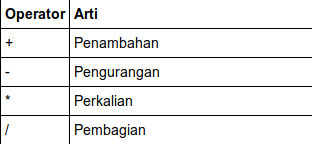
\includegraphics[width=6cm]{pip/aritmatika.png}
	\centering
	\end{figure}\\
	Kode yang digunakan untuk mengkonversikan integer(int) ke String(str)\\
	p=333 \#variabel\\
	string = str(p) \#konversi integer ke string\\ 
	print(string) \#mencetak hasil\\
	Kode yang digunakan untuk mengkonversikan String(str) ke integer(int)\\
	p=’333’\\
	integer = int(p) \#konversi string ke integer\\
	print(integer) \#mencetak hasil\\

	\item Syntax Perulangan\\
	Perulangan For adalah perulangan yang terhitung disebut juga counted loop\\
	Contoh Kode:\\	
	For indek in range(banyak\_perulangan)\\
	Penerapannya:\\
	Mengulang = 3\\
	For i in range(mengulang):\\
	Print “Mengulang ke –“+str(i)\\
	Hasil:\\
	Mengulang ke-0\\
	Mengulang ke-1\\
	Mengulang ke-2\\
	Mengulang ke-3\\
	\\
	\\
	Perulangan While adalah perulangan yang tidak terhitung disebut juga uncounted loop perulangan yang 		tidak tentu berapa perulangannya\\
	Contoh Kode:\\
	while (True):\\
	Penerapannya:\\
	Jawab = ‘ya’\\
	Hitung = 0\\
	while (True):\\
	Hitung += 1\\
	Jawab = raw\_input(“mengulangi lagi tidak?”)\\
	if jawab == ‘tidak’\\
	break \\
	print “total perulangan: “ + str(hitung)\\
	Hasil:\\
	Mengulangi lagi tidak? Ya\\
	Mengulangi lagi tidak?ya\\
	Mengulangi lagi tidak? Tidak\\ 
	Total perulangan: 3\\

	\item Jika kita terdapat di SATU keputusan syntax yang digunakan adalah if dengan kode sebagai 				berikut:\\
	if  lelah == “ya”:\\
  	  print(“beristirahatlah”)\\
	Hasil:\\
	Apakah kamu lelah? [ya/tidak]: ya\\
	Beristirahatlah\\
	Apakah kamu lelah?[ya/tidak]: tidak\\
	Jika kita terdapat di DUA keputusan syntax yang digunakan adalah if/Else dengan kode sebagai berikut:\\
	Umur = input(“Berapa umur kamu: “)\\
	if umur >= 17:\\
  	  print (“kamu boleh membuat KTP”)\\
	else:\\
  	  print(“kamu belum boleh membuat KTP”)\\
	Hasil:\\
	Berapa umur kamu: 18\\
	Kamu boleh membuat KTP\\
	Berapa umur kamu: 15\\
	Kamu belum boleh membuat KTP\\ 
	Jika kita terdapat di LEBIH DARI DUA keputusan menggunakan syntax if/elif/else dengan kode sebagai 			berikut:\\
	if nilai >= 95:\\
  	  grade =”A”\\
	elif nilai >=85:\\
  	  grade =”B+”\\
	elif nilai >=75:\\
  	  grade =”B”\\
	else:\\
  	  grade =”C”\\
	Hasil: \\
	Inputkan nilaimu : 98\\
	Grade A\\
	Inputkan nilaimu : 85\\
	Grade B+\\
	Inputkan nilaimu : 77\\
	Grade B\\
	Inputkan nilaimu: 72\\
	Grade C\\

	
	\item TypeError: unsupported operand type(s) for +: 'int' and 'str' penanganan error ini bisa 				ditangani menggunakan casting operand kedua menjadi integer\\
	TypeError: can only concatenate str (not "int") to str penanganan error ini bisa ditangani 					menggunakan casting operand kedua menjadi string
	
	\item Try Except adalah salah satu bentuk dari penanganan eror di python. Cara pemakaiannya adalah:\\
	Terdapat pembagaian suatu angka dengan nol (0) dan sesuai ketentuan akan terjadi eror. Oleh karena 			itu dapat dikurungkan dengan try except, lalu dikeluarkan erornya sampai tertangkap oleh except, yang 	harusnya tidak dapat di eksekusi tetap dapat dieksekusi tetapi akan muncul eror seperti dibawah ini:\\
	x = 0\\
	try:\\
  	  X = 3/0\\
	except exception, e:\\
  	  print e \\

	print x+1\\
	maka akan muncul integer division or modulo by zero 1 \\


\end{enumerate}
